\documentclass[11pt]{article}

\usepackage[margin=1in]{geometry}
\usepackage{amsmath}
\usepackage{amssymb}
\usepackage{booktabs}
\usepackage{graphicx}
\PassOptionsToPackage{hyphens}{url}
\usepackage[hidelinks]{hyperref}
\usepackage{enumitem}
\usepackage{caption}
\usepackage{natbib}

\newcommand{\Dthreeone}{D_{3/1}}
\newcommand{\Dfourone}{D_{4/1}}
\newcommand{\Qninefifty}{Q_{90/50}}
\newcommand{\Cg}{C_g}
\newcommand{\dRMSE}{\Delta\mathrm{RMSE}}

\title{Variance Constraints Do Not Improve Prediction of Subsequent
Insect Abundance Change: A Prospective Validation Across Long-Term
Monitoring Studies}
\author{Elias De Jes\'us \\ Independent Researcher \\ ORCID: 0009-0007-0190-9143}
\date{}

\begin{document}
\maketitle

\begin{abstract}
\noindent Higher-order variance structure has been proposed as a
diagnostic of ecological vulnerability distinct from variance magnitude,
but this proposition has not previously been tested prospectively. We
report a prospective, pre-registered validation of that hypothesis using
the van Klink et al.\ (2020) global database of long-term insect
assemblage changes (70{,}955 abundance/biomass observations, 1{,}663
plots, 166 studies, 1925--2018). Working from 1{,}613 candidate,
1{,}129 eligible abundance series (99 studies; $\geq$10 usable years,
chronologically split into an early predictor window and a held-out
future window before any predictor--outcome association was examined),
we tested three scale-invariant, higher-order constraint metrics ---
$\Dthreeone$, $\Dfourone$, and $\Qninefifty$ --- as predictors of each
series' subsequent abundance trend, using conventional baseline features
and grouped, study-aware cross-validation. None of the three metrics
showed the predicted direction after Holm correction (raw $p=0.905$,
$0.871$, $0.043$; Holm $p=1.000$, $1.000$, $0.171$). Adding all three to
a conventional baseline model did not improve out-of-sample prediction
(pooled RMSE: $M_0=0.16900$, $M_1=0.16932$; $\dRMSE=-0.00032$; only 4 of
10 folds favored the augmented model; permutation controls $p=0.454$ and
$p=0.583$). A separate, independently frozen prospective test of a
study-level, hierarchical meta-variability statistic ---
$\Cg=\mathrm{SD}_i(\mathrm{CV}_i)/\mathrm{Mean}_i(\mathrm{CV}_i)$,
computed from each study's own first 10 historical years and evaluated
against a fully held-out future period ($n=11$ effective study contexts
after a mandatory outcome-timing filter) --- likewise showed no
incremental predictive value (pooled RMSE: $M_0=0.141950$,
$M_1=0.144303$; $\dRMSE=-0.002354$; 10{,}000-permutation one-sided
$p=0.5304$). Taylor's Law was independently, strongly replicated as a
descriptive benchmark ($b=1.930$, $R^2=0.974$), confirming the dataset
itself is not featureless even though the tested constraint metrics
carried no incremental prospective information. Constraint-like variance
structure was measurable but did not provide incremental out-of-sample
information about subsequent abundance change beyond conventional
baseline features. These results support a conservative conclusion:
descriptive constraint structure should not be interpreted as ecological
vulnerability or early-warning information without prospective,
target-specific validation.
\end{abstract}

\noindent\textbf{Keywords:} insect decline, variance structure, prospective
validation, negative results, meta-variability, Taylor's Law, early-warning
indicators

\section{Introduction}

Global insect populations have experienced substantial declines over
recent decades, with estimates suggesting biomass reductions of 1--2\%
annually in some regions \citep{hallmann2017,vanklink2020a}. These
declines carry profound implications for ecosystem function, including
pollination services, nutrient cycling, and food web stability
\citep{potts2010,yang2014}. Accurate assessment of population health and
early detection of vulnerability are therefore important for conservation
planning and ecosystem management.

Conventional monitoring approaches typically focus on two primary
metrics: mean abundance trends and population variance. Mean trends
capture directional change but may detect stress only after substantial
population loss has occurred. Single-scale variance metrics, such as the
coefficient of variation (CV), describe population stability but do not
necessarily distinguish natural fluctuation regimes from pathological
instability \citep{inchausti2002,houlahan2007}.

A growing body of literature has suggested that higher-order variance
structure --- the distribution and coupling of variabilities across
populations, strata, and scales --- may contain diagnostic information
not captured by first-order statistics \citep{carpenter2006,scheffer2009}.
In particular, the variance of variances, or CV of CVs, has been proposed
as a candidate early-warning indicator for critical transitions in
complex systems \citep{dakos2012}. A companion idea is that ecological
vulnerability may not concentrate where variance is largest: highly
variable populations may possess intrinsic buffering capacity, while
populations with more constrained variance may represent bottlenecks
where perturbations amplify and propagate \citep{ives1999,tilman1999}.

Both ideas motivated an earlier, exploratory analysis of this same
database, which reported a bounded population-level CV-of-CVs estimate,
stratum-specific variance-structure contrasts, and proposed a family of
candidate early-warning metrics. That analysis was explicitly diagnostic
and correlational, and it called for validation on independent data and
prospective time series before any of its candidate indicators could be
treated as established. The present paper reports exactly that
validation, conducted as a separate, prospectively frozen research
program \emph{after} the exploratory analysis, using a discipline in
which every eligibility rule, predictor definition, outcome definition,
validation design, negative control, and support criterion was committed
to a version-controlled record \emph{before} any predictor--outcome
association was examined.

The central distinction this paper turns on is simple to state and easy
to blur in practice:

\begin{quote}
\emph{A statistical feature may describe constrained variability without
carrying information about a subsequent ecological outcome.}
\end{quote}

Measurability is not predictive value. A metric can be well-defined,
scale-invariant, and reproducibly estimable from real data --- as all of
the metrics tested here are --- and still carry zero incremental
information about what happens next in a specific series. Distinguishing
these two properties requires holding out the future: computing every
candidate predictor from an early historical window, and testing it only
against a later, disjoint outcome window that the predictor never saw.
This paper treats $\Dthreeone$, $\Dfourone$, $\Qninefifty$, and the
contextual meta-variability statistic $\Cg$ throughout as
\emph{prospectively tested candidate indicators}, not as established
vulnerability measures, and asks two falsifiable questions:

\begin{enumerate}[label=(\arabic*)]
\item Does a higher-order, scale-invariant constraint metric, measured in
an early historical window, predict a series' subsequent abundance trend,
beyond conventional baseline information?
\item Does a study-level, hierarchical historical meta-variability
statistic contain prospective information about subsequent abundance
change, beyond the same conventional baseline?
\end{enumerate}

\section{Data and Methods}

\subsection{Data provenance and scale}

The primary dataset is \citet{vanklink2020} (Knowledge Network for
Biocomplexity, DOI: \href{https://doi.org/10.5063/F11V5C9V}{10.5063/F11V5C9V},
CC~BY~4.0), independently downloaded and checksum-verified against the
provider's own reported checksums. The corpus contains \textbf{70{,}955}
abundance/biomass observations across \textbf{1{,}663} plots from
\textbf{166} original studies, spanning \textbf{1925--2018}, stratified
into six ecological strata (Air, Water, Herb layer, Soil surface, Trees,
Underground). These headline scale figures were independently
re-verified against the raw, checksum-verified files rather than assumed
from the source's own documentation.

The database aggregates heterogeneous monitoring designs: different
studies used different trapping methods, sampling intensities, and
reporting units. Raw abundance magnitudes are therefore \textbf{not}
treated as directly comparable across studies or locations. The entire
analysis instead focuses on within-series temporal structure (a series'
own coefficient of variation, its own higher-order dispersion, its own
temporal trend) and each series' own subsequent temporal change ---
quantities that are, by construction, invariant to a fixed multiplicative
difference in reporting scale between studies (\S\ref{sec:invariance}).
Biomass records exist in the source ($\mathrm{MetricAB}=$biomass) but are
excluded from the primary analysis entirely; abundance
($\mathrm{MetricAB}=$abundance) is the sole primary quantity, consistent
with the frozen protocol's own scope.

\subsection{Prospective design principle}

Every choice reported in this section --- eligibility, chronological
split, predictor and outcome definitions, model specification, validation
design, negative controls, multiplicity correction, and support criteria
--- was frozen and committed to a version-controlled protocol
\emph{before} any predictor--outcome association was computed. The
research chronology is:

\begin{center}
\begin{tabular}{@{}ll@{}}
\toprule
Commit & Content \\
\midrule
\texttt{21e6992} & Round 0: protocol freeze (eligibility, outcome, metrics, model, controls) \\
\texttt{206742f} & Round 1: primary H1/H2/H3 results (executed once) \\
\texttt{d3246d9} & Round 2A: CV-of-CVs \emph{feasibility} audit (no outcome touched) \\
\texttt{3e30670} & H4 protocol freeze (converts the feasibility recommendation into an immutable design) \\
\texttt{8d6db88} & H4: primary result (executed once) \\
\bottomrule
\end{tabular}
\end{center}

\subsection{Primary abundance-series construction and eligibility}

The unit of analysis is a longitudinal series keyed by
$(\mathrm{DataSource\_ID}, \mathrm{Plot\_ID}, \mathrm{Stratum})$,
restricted to abundance records. Of \textbf{1{,}613} candidate abundance
series, \textbf{1{,}129} were \emph{eligible}: $\geq 10$ usable years
(years with a non-null aggregated abundance value, summing multiple
within-year sampling periods before any further computation), spanning
\textbf{99} distinct studies.

Each eligible series' usable years were split chronologically into an
early predictor window (the first $\lceil n/2 \rceil$ years) and a held-out
future window (the remaining $\lfloor n/2 \rfloor$ years), guaranteeing
$\geq 5$ years in each window. No later-window observation was used in
predictor construction at any point; this was enforced both structurally
(the split is defined by ordering years, not calendar arithmetic) and by
an explicit programmatic leakage check.

\subsection{Predictors}

\paragraph{Conventional baseline (M0).} Five features computed from the
early window alone: mean $\log(1+\mathrm{abundance})$, coefficient of
variation, OLS temporal trend of $\log(1+\mathrm{abundance})$ on year,
number of usable years, and temporal span.

\paragraph{Constraint metrics.} For a series' early-window abundance
values $\{x_1,\dots,x_n\}$, define the power mean of order $p$,
\[
M_p = \left(\frac{1}{n}\sum_{i=1}^{n} x_i^{\,p}\right)^{1/p}.
\]
The three frozen constraint candidates are
\[
\Dthreeone = \frac{M_3}{M_1}, \qquad
\Dfourone = \frac{M_4}{M_1}, \qquad
\Qninefifty = \frac{Q_{0.90}}{Q_{0.50}},
\]
where $Q_q$ denotes the $q$-quantile. By the power-mean inequality,
$M_p \geq M_1$ for $p>1$ with equality iff $x$ is constant, so all three
metrics attain their minimum value of 1 exactly at zero within-series
dispersion (the ``tightest'' possible constraint) and increase with
dispersion.

\subsubsection{Scale invariance}
\label{sec:invariance}
For any $c>0$, $M_p(c\,x) = c\,M_p(x)$, so $\Dthreeone$ and $\Dfourone$
are invariant to multiplicative rescaling of a series' raw abundance;
quantiles scale identically under $c>0$, so $\Qninefifty$ is invariant by
the same argument. This property is what licenses comparing these
metrics across studies recorded on different, unknown raw scales.

\subsection{Validation design}

Because series within a study share methodology, observers, and regional
drivers, random row-wise cross-validation is invalid. All Round~1
inference used \textbf{10-fold GroupKFold}, grouped by
$\mathrm{DataSource\_ID}$, so no study's series ever appear in both the
training and test partition of a fold. Model $M_0$ uses the five baseline
features; $M_1$ uses $M_0$ plus one (H1) or all three (H2) constraint
metrics. Standardization is fit on the training fold only; a Ridge
fallback ($\alpha=1$) is used only if a training design matrix's
condition number exceeds $10^8$.

\subsection{H1 / H2 and multiplicity}

\textbf{H1} (per metric): does the metric's early-window value predict
the frozen direction of the later-window trend, individually, after study
clustering? Evaluated via a cluster-robust ($\mathrm{DataSource\_ID}$)
OLS coefficient. \textbf{H2}: does adding all three metrics to $M_0$
improve pooled out-of-fold RMSE ($\dRMSE = \mathrm{RMSE}(M_0)-
\mathrm{RMSE}(M_1)$, positive favors the constraint metrics)? Four tests
(H1-$\Dthreeone$, H1-$\Dfourone$, H1-$\Qninefifty$, H2) form one
predeclared Holm family at $\alpha=0.05$.

\subsection{Negative controls}

Three controls, 2{,}000 permutations each: \textbf{NC1} permutes each
constraint metric within study; \textbf{NC2} permutes the future outcome
within study; \textbf{NC3} reverses the early/late window roles as a
leakage diagnostic (not a hypothesis test).

\subsection{Prospective test of contextual meta-variability (H4)}

A population-level CV-of-CVs is a single number and cannot, by itself,
predict which individual series will decline more than another. A
\emph{prospective}, context-varying version requires a group-level,
time-indexed statistic, computed from multiple contemporaneous series
sharing a context. A separate feasibility audit (Round~2A, \texttt{d3246d9})
established, \emph{without ever touching any outcome value}: LEVEL
(a single historical estimate per context) was marginally feasible;
CHANGE (a temporal slope of the statistic) was underpowered at every
tested multiplicity (3--14 of 99 studies, depending on threshold);
constituent-group sizes below 15 series showed materially unstable
estimator behavior (95\% bootstrap CI width $\geq 0.49$ even at 30
constituent series, with a single extreme constituent CV still shifting
the group estimate by $\sim$0.33 on average); and the correct inferential
scale is the (study, historical-window) pair, never the plot or series
count broadcast onto it.

This feasibility recommendation was converted into an immutable protocol
(\texttt{3e30670}) before any H4 result was computed. For a study's
constituent series $i$ with early-window abundance $x_i$,
\[
\mathrm{CV}_i = \frac{\mathrm{SD}_i}{\mathrm{Mean}_i}, \qquad
\Cg = \frac{\mathrm{SD}_i(\mathrm{CV}_i)}{\mathrm{Mean}_i(\mathrm{CV}_i)}.
\]
$\Cg$ is \textbf{contextual}: it is defined per study and is never
treated as, or tested as, a universal constant. The historical window is
the first 10 elements of the sorted, deduplicated \emph{union} of usable
years across a study's eligible series (rank-based, not calendar
arithmetic); adequacy requires $\geq 15$ constituent series with $\geq 2$
observations in that window. Chronology follows Design~C: this fixed
10-year window, then \emph{all} remaining years as a fully held-out
future period. A series may contribute an outcome only if its own
Round~1 late window (unchanged formula,
$\texttt{ols\_trend\_slope}(\log(1+\mathrm{Number}),\,\mathrm{Year})$)
falls strictly after the study's H4 cutoff --- the unique condition
required to keep the historical-to-future arrow honest, given that a
series' own Round~1 split need not align with the study-level H4 cutoff.

Validation is \textbf{leave-one-study-out} (LOSO; the parameter-free
generalization of GroupKFold once the number of eligible groups is much
smaller than Round~1's 99). The primary statistic is pooled LOSO
$\dRMSE = \mathrm{RMSE}(M_0)-\mathrm{RMSE}(M_1)$, with $M_1 = M_0 + \Cg$.
Inference uses a \textbf{between-study permutation} of the
study-to-$\Cg$ mapping (the valid adaptation of Round~1's NC1/NC2 to a
study-level, not series-level, predictor): 10{,}000 permutations, seed
20260907, one-sided, $p=(1+\#\{b:\Delta_{\mathrm{perm},b}\geq
\Delta_{\mathrm{obs}}\})/10001$. Direction was predeclared \emph{before}
any outcome was inspected, by direct analogy to Round~1's own H1
convention: a lower (tighter) historical $\Cg$ was predicted to predict a
worse future trend (positive coefficient sign).

\section{Results}

\subsection{Validation population}

\begin{table}[h]
\centering
\caption{Dataset and validation population.}
\begin{tabular}{@{}lr@{}}
\toprule
Quantity & Value \\
\midrule
Total observations & 70{,}955 \\
Plots & 1{,}663 \\
Studies (source-level) & 166 \\
Year coverage & 1925--2018 \\
Candidate abundance series & 1{,}613 \\
Round 1 eligible series ($\geq$10 usable years) & 1{,}129 \\
Eligible studies & 99 \\
Common analysis sample (H1/H2) & 1{,}126 series / 99 studies \\
H4 structurally adequate study-windows ($\geq$15 constituents) & 16 \\
H4 effective study $N$ (after outcome-timing filter) & 11 \\
\bottomrule
\end{tabular}
\end{table}

\subsection{H1: individual constraint metrics}

None of the three metrics showed the predicted direction after
correction (Table~\ref{tab:h1}). $\Qninefifty$'s raw $p=0.043$ must
\textbf{not} be read as a near-significant positive result: its estimated
direction was opposite the frozen prediction, and Holm correction leaves
$p=0.171$.

\begin{table}[h]
\centering
\caption{H1 results: individual constraint metrics.}
\label{tab:h1}
\begin{tabular}{@{}lccccc@{}}
\toprule
Metric & Predicted direction met? & Raw $p$ & Holm $p$ & Verdict \\
\midrule
$\Dthreeone$ & No & 0.905 & 1.000 & Not supported \\
$\Dfourone$ & No & 0.871 & 1.000 & Not supported \\
$\Qninefifty$ & No & 0.043 & 0.171 & Not supported \\
\bottomrule
\end{tabular}
\end{table}

\subsection{H2: incremental out-of-sample prediction}

Adding $\Dthreeone$, $\Dfourone$, and $\Qninefifty$ to the conventional
baseline did not improve, and slightly worsened, out-of-fold prediction
(Table~\ref{tab:h2}, Figure~\ref{fig:round1folds}). Only 4 of 10 folds
favored $M_1$. Both negative controls placed the observed $\dRMSE$ well
inside their permutation null distributions (NC1 $p=0.454$; NC2
$p=0.583$; 2{,}000 permutations each). NC3 (time-reversal diagnostic)
showed no leakage artifact. Holm-adjusted $p=1.000$.

\begin{table}[h]
\centering
\caption{Round 1 model performance, $M_0$ vs.\ $M_1$.}
\label{tab:h2}
\begin{tabular}{@{}lcc@{}}
\toprule
Model & Pooled out-of-fold RMSE & \\
\midrule
$M_0$ (baseline) & 0.16900 & \\
$M_1$ (baseline + $\Dthreeone,\Dfourone,\Qninefifty$) & 0.16932 & \\
\midrule
$\dRMSE = \mathrm{RMSE}(M_0)-\mathrm{RMSE}(M_1)$ & $-0.00032$ & (folds favoring $M_1$: 4/10) \\
\bottomrule
\end{tabular}
\end{table}

\begin{figure}[h]
\centering
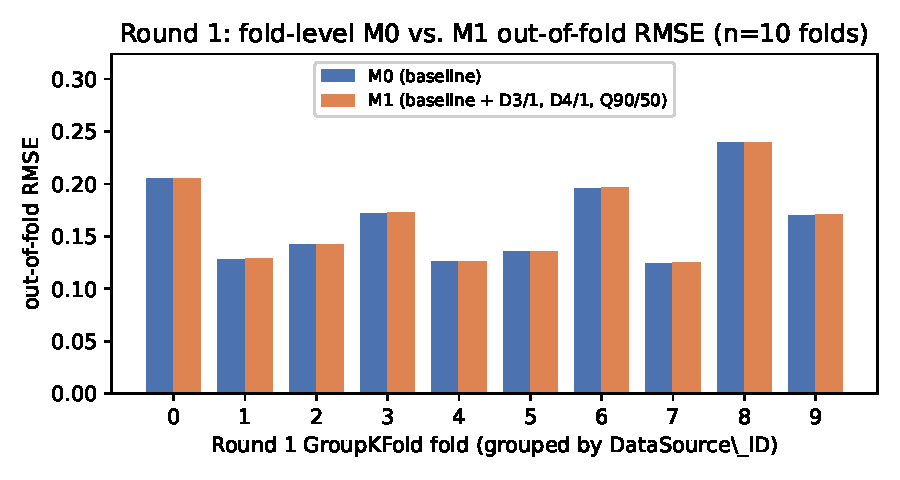
\includegraphics[width=0.75\textwidth]{figures/round1_fold_rmse.pdf}
\caption{Round 1 fold-level out-of-fold RMSE, $M_0$ vs.\ $M_1$, across the
10 GroupKFold folds. Reproduced from \texttt{results/round1\_primary\_results.json}
(commit \texttt{206742f}); no new analysis was run to produce this figure.}
\label{fig:round1folds}
\end{figure}

\textbf{Adding $\Dthreeone$, $\Dfourone$, and $\Qninefifty$ did not
improve prediction of subsequent abundance trends beyond the conventional
baseline.}

\subsection{Secondary stratum analysis}

Only the four strata passing the frozen adequacy gate ($\geq$30 eligible
series and $\geq$5 independent studies) were inferentially tested: Air,
Water, Herb layer, Soil surface. Trees and Underground failed the gate
and were not tested. Direction was \textbf{not} consistent across strata,
and constraint metrics made prediction of subsequent trends
\emph{materially worse} in two of the four:

\begin{itemize}
\item Herb layer: $\dRMSE \approx -0.041$
\item Soil surface: $\dRMSE \approx -0.051$
\item Air: $\dRMSE \approx +0.0001$ (negligible)
\item Water: $\dRMSE \approx -0.0014$
\end{itemize}

This is a secondary, uncorrected result and is never promoted to the
primary conclusion. It does \textbf{not} support treating Herb layer or
Soil surface as validated vulnerability bottlenecks, nor Air or Water as
validated buffers.

\subsection{H4: prospective contextual meta-variability}

Of 99 candidate studies, \textbf{16} were structurally adequate (a fixed
10-year historical window containing $\geq 15$ constituent series).
Applying the frozen outcome-timing filter --- required so that every
contributing series' future outcome genuinely postdates the study's
historical cutoff --- left an \textbf{effective study $N=11$}. This is
below the $\sim$19--20 studies estimated during the Round~2A feasibility
audit; that estimate predated the outcome-timing filter, which was
derived only when the H4 protocol itself was frozen, and $N=11$, not
$N\approx 19$--20, is the number that supported the executed test. $N=11$
clears the frozen floor of 10 below which the result would have been
declared uninterpretable/blocked.

Across these 11 studies, $\Cg$ ranged from 0.2503 to 0.5606 (mean
0.4277, SD 0.0788, median 0.4056) --- real, non-degenerate, contextual
values, reported without removal, winsorization, or transformation.

\begin{table}[h]
\centering
\caption{H4 prospective result.}
\label{tab:h4}
\begin{tabular}{@{}lc@{}}
\toprule
Quantity & Value \\
\midrule
Effective study $N$ & 11 \\
$\mathrm{RMSE}(M_0)$ & 0.141950 \\
$\mathrm{RMSE}(M_1)$ & 0.144303 \\
$\dRMSE$ & $-0.002354$ \\
LOSO folds favoring $M_1$ & 7 / 11 \\
Secondary standardized $\Cg$ coefficient & $+0.00875$ (correct sign; cluster-robust $p=0.4423$) \\
Permutation $p$ (10{,}000 draws, one-sided) & 0.5304 \\
\bottomrule
\end{tabular}
\end{table}

Seven of 11 LOSO folds individually favored $M_1$, yet pooled performance
still favored $M_0$ (Table~\ref{tab:h4}): a majority of folds showing a
small favorable shift does not override pooled error when one fold (a
single study) carries a large unfavorable shift ($\dRMSE_{\text{fold}}
\approx -0.063$ for that study alone). The secondary standardized $\Cg$
coefficient had the predicted sign but was not significant under
asymptotic cluster-robust inference; per the frozen protocol, this
secondary result cannot rescue a failed primary criterion. The
10{,}000-permutation test (Figure~\ref{fig:h4perm}) placed the observed
$\dRMSE$ near the null median (null mean $-0.00317$, SD $0.00474$;
$q_{05}=-0.01267$, $q_{50}=-0.00208$, $q_{95}=0.00320$), giving
$p=0.5304$ --- far from the frozen $\alpha=0.05$ threshold in either
direction.

\begin{figure}[h]
\centering
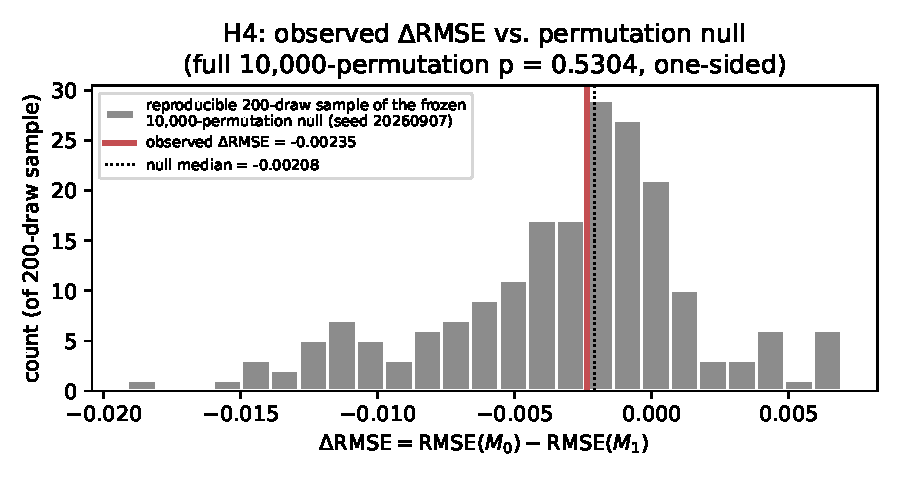
\includegraphics[width=0.75\textwidth]{figures/h4_permutation_null.pdf}
\caption{H4: observed $\dRMSE$ against a reproducible 200-draw sample of
the frozen 10{,}000-permutation null distribution (full summary
statistics computed from all 10{,}000 permutations; commit
\texttt{8d6db88}). No new permutation analysis was run to produce this
figure.}
\label{fig:h4perm}
\end{figure}

\textbf{Frozen verdict: NOT SUPPORTED.}

\subsection{Descriptive benchmarks}

\subsubsection{CV-of-CVs}

The exploratory manuscript this validation program tests reported a
population-level $\mathrm{CV}_{\mathrm{CVs}} \approx 0.610$. An
independent recomputation under this project's own transparent,
disclosed methodology gave \textbf{0.512} --- in the same general range,
but not an exact reproduction (the original code and exact filtering
choices were not available to this project). Neither value is treated as
universal. A finite empirical CV-of-CVs establishes only finite
dispersion in the specific population it was computed from; it does
\textbf{not}, by itself, establish an ecological bound, a sampling
artifact, or predictive value --- these are four logically distinct
claims, and only the first follows automatically from a finite number.
The prospective H4 test above did not demonstrate that historical,
contextual CV-of-CVs improves prediction of subsequent abundance change.
\textbf{Measurability is not universality, and descriptive structure is
not predictive information.}

\subsubsection{Taylor's Law}

Log--log regression of within-series variance against within-series mean
across eligible series gave $b=1.930$, $R^2=0.974$ --- close to, though
not assumed identical to, the exploratory manuscript's reported
$b\approx1.959$, $R^2\approx0.962$. This is a strong, independently
reproduced descriptive regularity, confirming the dataset is not
featureless. It is \textbf{not} evidence that the tested constraint
metrics predict vulnerability, and no time-varying ``Taylor exponent
shift'' statistic was ever defined or tested in this program; any such
claim in the exploratory manuscript remains untested.

\section{Discussion}

The predeclared higher-order variance metrics --- $\Dthreeone$,
$\Dfourone$, $\Qninefifty$, and the independently frozen contextual
statistic $\Cg$ --- were all measurable, reproducible, and scale-invariant
by construction. None added incremental prospective information about
subsequent abundance change beyond conventional baseline features, under
either of two independently designed, differently scaled prospective
tests. This is the central result of this paper.

\subsection{Measurable structure versus target-specific information}

A recurring temptation in this literature is to read descriptive
structure --- a tight variance regime, a bounded CV-of-CVs, a particular
Taylor exponent --- directly as an ecological signal. The results here
illustrate why that step needs its own evidence: \emph{structural
tightness alone is insufficient evidence of ecological vulnerability}.
This is not a universal theorem about all possible constraint metrics in
all possible systems; it is what was found for the three specific,
predeclared metrics and the one specific, predeclared contextual
statistic tested in this specific dataset and design.

\subsection{Why the null results matter}

A negative result under a design this disciplined is informative, not
merely an absence of finding. It shows that a descriptive pattern
observed in one analysis (the original, exploratory stratified variance
contrasts) does not automatically survive being asked a sharper, prospective
question of the same data. It highlights a hierarchical effective-sample-size
problem (\S\ref{sec:effectiveN}) that a purely descriptive analysis of the
same corpus could not have exposed. It demonstrates, concretely, why
chronological, study-aware validation is stricter than cross-sectional
comparison: Round 1's own grouped cross-validation and H4's leave-one-study-out
design are both engineered specifically to prevent the kind of
pseudoreplication that a naive plot-level or observation-level analysis of
this corpus would risk. And the negative controls (NC1--NC3, and H4's
between-study permutation) directly support the interpretation that there
is no detectable incremental signal in the tested metrics, rather than
merely an absence of statistical significance under one particular model.

\subsection{Effective sample size}
\label{sec:effectiveN}

The database contains 70{,}955 observations and 1{,}663 plots. H4's final
inferential test ultimately rested on \textbf{11} effective study
contexts. This is not a contradiction or a design flaw --- it is the
direct, unavoidable consequence of testing a \emph{hierarchical,
study-level} predictor: $\Cg$ does not vary within a study, so no amount
of within-study replication (plots, series, observations) increases the
number of independent points at which $\Cg$ itself varies. Large raw
observational $N$ does not imply large inferential $N$ for a contextual
predictor of this kind. This is a substantive methodological finding in
its own right, distinct from the negative result itself: a future study
proposing a contextual, hierarchical early-warning statistic should
budget its expected effective $N$ at the level the predictor actually
varies at, not at the level the raw corpus happens to report. The H4 test
reported here should accordingly be read as \emph{prospectively
specified but small-effective-$N$}, not as strongly powered; failure to
support H4 is evidence against a detectable predictive effect
\emph{under this specific design}, not proof that no ecological
relationship of this kind could ever exist at a larger, more richly
sampled effective $N$.

\section{Limitations}

\begin{itemize}
\item The source database aggregates heterogeneous monitoring designs
(sampling methods, units, durations) across originally independent
studies.
\item All analyses are observational; no causal claim is made or
licensed by any result in this paper.
\item Subsequent abundance trend is one operationalization of ecological
vulnerability among several plausible ones; a null result for this
outcome does not test other outcomes (e.g.\ local extinction, biomass
decline, food-web disruption).
\item Round 1's effective study $N$ (99) and H4's effective study $N$
(11) differ by an order of magnitude, for the structural reasons given in
\S\ref{sec:effectiveN}.
\item The $\Cg$ estimator showed material single-value sensitivity even
at its largest tested constituent-group sizes (Round 2A).
\item Study structure is unequal: which studies meet H4's adequacy gate
is itself correlated with a study's own plot count, a design artifact
rather than an ecological one (Round 2A).
\item No causal inference, no claim of a universal CV-of-CVs constant or
ecological bound, no real-time forecasting validation, and no
independent external-dataset validation are made anywhere in this paper.
\end{itemize}

These limitations qualify the scope of the negative result; they do not
undermine its validity. The result stands as: under this specific,
prospectively frozen design, on this specific dataset, these specific
metrics did not add prospective predictive value.

\section{Future Work (untested extensions)}

The exploratory manuscript this program validates included two
cross-domain illustrations that are \textbf{not} part of, and do not
provide evidence for, the primary result above.

\textbf{Bioacoustic classification data} (Cicadidae/Orthoptera species
classification samples) were never incorporated into any frozen protocol
in this validation program and remain an \textbf{untested} extension ---
a plausible future automated-monitoring application, not validating
evidence.

\textbf{Paleontological (Paleozoic chondrichthyan) cross-scale
comparison} was likewise never tested in this program and remains an
\textbf{untested} cross-scale analogy. Neither extension is treated as
confirming, illustrating, or generalizing the primary result in any of
the sections above.

\section{Conservation implications}

The prospective validation reported here does \textbf{not} support
directing conservation attention toward Herb layer, Soil surface, or
Underground strata on the basis of the tested constraint metrics, nor
toward Air or Water strata as validated buffers (\S3.3). A more
defensible statement, given the evidence in this paper, is: variance-structure
metrics of the kind tested here should not be used for conservation
prioritization without independent, prospective, target-specific
validation.

\section{Epistemic Status}

\textbf{Supported:} the source dataset's scale and provenance; the
eligible validation populations (Round 1: 1{,}129 series/99 studies; H4:
11 effective study contexts); strong Taylor's Law scaling as a
descriptive benchmark; reproducibility of every frozen analysis
(123 tests passing at the final H4 state); contextual measurability of
CV-of-CVs (as $\Cg$, a real, computable, per-study quantity).

\textbf{Not supported:} $\Dthreeone$, $\Dfourone$, and $\Qninefifty$ as
vulnerability predictors; incremental predictive advantage of the Round~1
constraint metrics over conventional baseline features; contextual
$\Cg$'s prospective early-warning value; the Herb-layer/Soil-surface
bottleneck interpretation; the Air/Water buffer interpretation; a
universal CV-of-CVs constant or ecological bound.

\textbf{Underpowered:} temporal CHANGE in CV-of-CVs (3--14 of 99 studies
depending on threshold; excluded from H4 by design).

\textbf{Untested:} any causal mechanism; the bioacoustic extension; the
paleontological extension; real-time forecasting utility; generalization
to any external, independently collected dataset.

\section{Conclusion}

$\Dthreeone$, $\Dfourone$, and $\Qninefifty$ did not improve prospective
prediction of subsequent insect abundance change beyond a conventional
baseline. An independently, separately frozen prospective test of
contextual historical CV-of-CVs likewise failed to demonstrate incremental
predictive value. Taylor's Law scaling remained a strong, independently
reproduced descriptive feature of the same dataset, confirming that the
null results above are not an artifact of an otherwise unstructured
corpus. Descriptive constraint structure should not be interpreted as
ecological vulnerability without demonstrated, target-specific predictive
information.

These results support a conservative distinction between descriptive
variance structure and ecological predictive information.
Constraint-like statistical organization may be measurable without
functioning as an early-warning indicator, and its ecological
significance should therefore be established prospectively rather than
inferred from structural tightness alone.

\section{Reproducibility and Data Availability}

All frozen protocols, execution code, tests, and results referenced in
this paper are version-controlled in the public GitHub repository,
\emph{insect-variance-constraint-validation}\footnote{\url{https://github.com/innerlightr-wq/insect-variance-constraint-validation}},
the living, version-controlled computational record for this work. A
permanent, citable archival deposit of this manuscript is separately
held on Zenodo\footnote{\url{https://doi.org/10.5281/zenodo.22646397}}
(De~Jes\'us, 2026); the Zenodo DOI is the version of record for citation
purposes, while the GitHub repository is the record to consult for the
current state of the code, tests, and results. The commit that produced
this manuscript revision is \texttt{f37a7b3}, itself built entirely from
the frozen, already-executed research chronology below (\texttt{f37a7b3}
is a post-hoc manuscript-writing commit, not part of that pre-result
freeze sequence). The full research chronology:

\begin{center}
\begin{tabular}{@{}ll@{}}
\toprule
\texttt{21e6992} & Round 0 protocol freeze \\
\texttt{206742f} & Round 1 results \\
\texttt{d3246d9} & CV-of-CVs feasibility audit \\
\texttt{3e30670} & H4 protocol freeze \\
\texttt{8d6db88} & H4 results \\
\bottomrule
\end{tabular}
\end{center}

123 tests were passing at the final H4 state referenced above. This count
is reported as reproducibility information only, not as scientific
evidence for or against any hypothesis in this paper.

The primary dataset \citep{vanklink2020} is licensed CC~BY~4.0; it is not
redistributed by this repository (raw third-party data is never
committed, per repository policy), but is fully re-downloadable and
checksum-verifiable from its original source using the commands and
checksums recorded in the repository's own data-provenance
documentation. This repository uses a dual license for its own original
content: original software/code is released under the MIT License, and
original manuscript text, documentation, and figures (including this
manuscript) are released under the Creative Commons Attribution 4.0
International License (CC~BY~4.0). Neither license extends to, or
relicenses, the third-party insect monitoring dataset above, which
remains governed solely by its own original CC~BY~4.0 terms as an
independent, externally authored dataset.

\bibliographystyle{plainnat}
\begin{thebibliography}{99}

\bibitem[Carpenter and Brock(2006)]{carpenter2006}
Carpenter, S.R.\ and Brock, W.A.\ (2006). Rising variance: a leading
indicator of ecological transition. \emph{Ecology Letters}, 9(3), 311--318.

\bibitem[Dakos et al.(2012)]{dakos2012}
Dakos, V., Carpenter, S.R., Brock, W.A., Ellison, A.M., Guttal, V., Ives,
A.R., K\'efi, S., Livina, V., Seekell, D.A., van Nes, E.H.\ and Scheffer,
M.\ (2012). Methods for detecting early warnings of critical transitions
in time series illustrated using simulated ecological data. \emph{PLoS
ONE}, 7(7), e41010.

\bibitem[Hallmann et al.(2017)]{hallmann2017}
Hallmann, C.A., Sorg, M., Jongejans, E., Siepel, H., Hofland, N., Schwan,
H., Stenmans, W., M\"uller, A., Sumser, H., H\"orren, T.\ and Goulson, D.\
(2017). More than 75 percent decline over 27 years in total flying insect
biomass in protected areas. \emph{PLoS ONE}, 12(10), e0185809.

\bibitem[Houlahan et al.(2007)]{houlahan2007}
Houlahan, J.E., Currie, D.J., Cottenie, K., Cumming, G.S., Ernest,
S.K.M., Findlay, C.S., Fuhlendorf, S.D., Gaedke, U., Legendre, P.,
Magnuson, J.J.\ and McArdle, B.H.\ (2007). Compensatory dynamics are rare
in natural ecological communities. \emph{Proceedings of the National
Academy of Sciences}, 104(9), 3273--3277.

\bibitem[Inchausti and Halley(2002)]{inchausti2002}
Inchausti, P.\ and Halley, J.\ (2002). The long-term temporal variability
and spectral colour of animal populations. \emph{Evolutionary Ecology
Research}, 4(7), 1033--1048.

\bibitem[Ives et al.(1999)]{ives1999}
Ives, A.R., Gross, K.\ and Klug, J.L.\ (1999). Stability and variability
in competitive communities. \emph{Science}, 286(5439), 542--544.

\bibitem[Potts et al.(2010)]{potts2010}
Potts, S.G., Biesmeijer, J.C., Kremen, C., Neumann, P., Schweiger, O.\ and
Kunin, W.E.\ (2010). Global pollinator declines: trends, impacts and
drivers. \emph{Trends in Ecology \& Evolution}, 25(6), 345--353.

\bibitem[Scheffer et al.(2009)]{scheffer2009}
Scheffer, M., Bascompte, J., Brock, W.A., Brovkin, V., Carpenter, S.R.,
Dakos, V., Held, H., Van Nes, E.H., Rietkerk, M.\ and Sugihara, G.\
(2009). Early-warning signals for critical transitions. \emph{Nature},
461(7260), 53--59.

\bibitem[Taylor(1961)]{taylor1961}
Taylor, L.R.\ (1961). Aggregation, variance and the mean. \emph{Nature},
189(4766), 732--735.

\bibitem[Tilman(1999)]{tilman1999}
Tilman, D.\ (1999). The ecological consequences of changes in
biodiversity: a search for general principles. \emph{Ecology}, 80(5),
1455--1474.

\bibitem[van Klink et al.(2020a)]{vanklink2020a}
van Klink, R., Bowler, D.E., Gongalsky, K.B., Swengel, A.B., Gentile, A.\
and Chase, J.M.\ (2020). Meta-analysis reveals declines in terrestrial
but increases in freshwater insect abundances. \emph{Science}, 368(6489),
417--420.

\bibitem[van Klink et al.(2020b)]{vanklink2020}
van Klink, R., Bowler, D.E., Chase, J.M., Comay, O., Driessen, M.M.,
Ernest, S.K.M., Gentile, A., Gilbert, F., Gongalsky, K., Owen, J., Pe'er,
G., Pe'er, I., Resh, V.H., Rochlin, I., Schuch, S., Swengel, A.E.,
Swengel, S.R., Valone, T.L., Vermeulen, R., Wepprich, T.\ and Wiedmann, J.\
(2020). A global database of long-term changes in insect assemblages.
Knowledge Network for Biocomplexity.
\url{https://doi.org/10.5063/F11V5C9V}

\bibitem[Yang and Gratton(2014)]{yang2014}
Yang, L.H.\ and Gratton, C.\ (2014). Insects as drivers of ecosystem
processes. \emph{Current Opinion in Insect Science}, 2, 26--32.

\end{thebibliography}

\end{document}
